\subsubsection{UC7 - Acquisto beni}
\begin{figure}[h]
	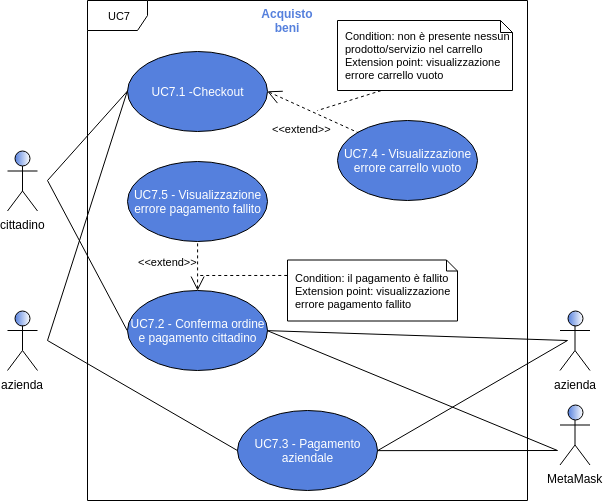
\includegraphics[width=14cm]{res/images/UC7-Generale.png}
	\centering
	\caption{Acquisto dei beni all'interno della piattaforma}
\end{figure}
\begin{itemize}
	\item \textbf{Attori Primari}: cittadino e azienda-cliente;
	\item \textbf{Attori Secondari}: azienda-venditrice, MetaMask\glo;
	\item \textbf{Descrizione}: i cittadini e le aziende possono acquistare i prodotti/servizi che avevano precedentemente aggiunto nel carrello;
	\item \textbf{Scenario}: l'utente innanzitutto inserisce dei prodotti nel carrello [UC6.1]. Dunque procede al checkout [UC7.1] dei prodotti nel carrello:
	\begin{itemize}
		\item i cittadini procedono con la conferma dell'ordine ed il pagamento immediato [UC7.2];
		\item le aziende invece dovono scegliere un metodo di pagamento [UC7.3.1] tra il pagamento immediato [UC7.3.2] ed il pagamento dilazionato [UC7.3.3]. A differenza dei cittadini, devono successivamente approvare la proposta d'ordine dal proprio account per ottenere la fatturazione.
	\end{itemize}
	
	\item \textbf{Precondizione}: il sistema ha reso disponibile all'utente l'utilizzo del carrello per poter effettuare degli acquisti. L'utente ha inserito degli oggetti nel carrello ed ha espresso la volontà di acquistare tali prodotti;
	\item \textbf{Postcondizione}: è stato effettuato l'acquisto dei beni presenti nel carrello. Se l'utente è cittadino, allora l'ordine è concluso e viene effettuato il pagamento all'azienda venditrice. Viceversa, nel caso il cliente fosse un'azienda, viene inviata una proposta d'ordine nella pagina dedicata, che dovrà successivamente essere confermata. Inoltre, nel caso questo fosse un ordine con pagamento immediato, il sistema provvederà a trattenere i soldi dovuti all'azienda venditrice finché non verrà confermata la correttezza della proposta della fattura.
\end{itemize} 
\subsubsection{UC7.1 - Checkout}
\begin{itemize}
	\item \textbf{Attori Primari}: cittadino, azienda;
	\item \textbf{Descrizione}: l'utente effettua il checkout per poter poi acquistare i prodotti inseriti nel carrello;
	\item \textbf{Scenario}: l'utente preme il pulsante per effettuare il checkout;
	\item \textbf{Inclusioni}: 
	\begin{itemize}
		\item \textbf{UC7.6}: l'utente inserisce l'indirizzo di spedizione;
	\end{itemize}
	\item \textbf{Estensioni}: 
	\begin{itemize}
		\item \textbf{UC7.4}: l'utente preme il pulsante di checkout senza aver ancora inserito almeno un prodotto/servizio nel carrello;
	\end{itemize}
	\item \textbf{Precondizione}: il sistema ha reso disponibile il carrello all'utente, identificandolo quindi come cittadino o azienda. L'utente ha espresso la volontà di procedere con il checkout premendo l'apposito pulsante;
	\item \textbf{Postcondizione}: l'utente accede alla pagina dove poter confermare l'acquisto e procedere con il pagamento.
\end{itemize}

\subsubsection{UC7.2 - Conferma ordine e pagamento cittadino}
\begin{itemize}
	\item \textbf{Attori Primari}: cittadino;
	\item \textbf{Attori Secondari}: azienda-venditrice, MetaMask\glo;
	\item \textbf{Descrizione}: l'utente visualizza il contenuto del carrello ed ha la possibilità di confermare l'ordine e procedere al pagamento che avviene attraverso l'utilizzo del plugin Metamask\glo;
	\item \textbf{Scenario}: l'utente preme il pulsante per effettuare il checkout;
	\item \textbf{Inclusioni}: 
	\begin{itemize}
		\item \textbf{UC6.2}: l'utente visualizza un riepilogo di tutti i prodotti presenti all'interno del carrello.
	\end{itemize}
	\item \textbf{Estensioni}: 
	\begin{itemize}
		\item \textbf{UC7.5}: l'utente tenta il pagamento ma l'esito non va a buon fine. La causa del fallimento dell'operazione è gestito dal plugin stesso.
	\end{itemize}
	\item \textbf{Precondizione}: il sistema ha reso disponibile il riepilogo dei prodotti con la possibilità di effettuare la conferma dell'ordine ed il pagamento. Almeno un elemento era stato inserito nel carrello; 
	\item \textbf{Postcondizione}: l'utente ha portato a termine la procedura di acquisto dei prodotti/servizi presenti nel carrello. L'azienda venditrice ha ricevuto il pagamento dal cliente e l'ordine è aggiunto alla lista delle fatture dell'azienda. Al cliente viene segnalato il successo dell'operazione.
\end{itemize}
\subsubsection{UC7.3 - Pagamento aziendale}
\begin{figure}[H]
	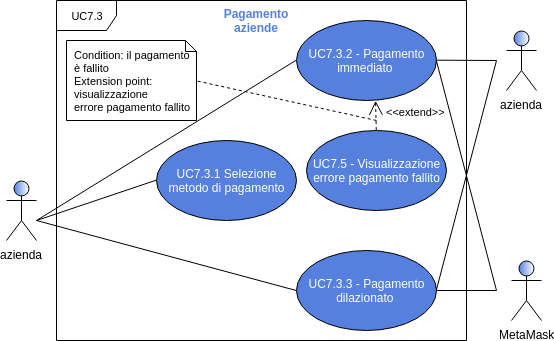
\includegraphics[width=14cm]{res/images/UC7-PagamentoAzienda.png}
	\centering
	\caption{Procedura di pagamento da parte delle aziende}
\end{figure}
\begin{itemize}
	\item \textbf{Attori Primari}: azienda-cliente;
	\item \textbf{Attori Secondari}: azienda-venditrice, MetaMask\glo;
	\item \textbf{Descrizione}: le aziende hanno un processo di pagamento differente dai cittadini, possono scegliere fra pagamento immediato e dilazionato\glo;
	\item \textbf{Scenario}: l'azienda sceglie un metodo di pagamento [UC7.3.1] tra il pagamento immediato [UC7.3.2] ed il pagamento dilazionato [UC7.3.3]. Successivamente dovrà approvare la proposta d'ordine dal proprio account per ottenere la fatturazione.
	\item \textbf{Inclusioni}: 
	\begin{itemize}
		\item \textbf{UC6.2}: l'utente visualizza un riepilogo di tutti i prodotti presenti all'interno del carrello.
	\end{itemize}
	\item \textbf{Precondizione}: il sistema ha reso disponibile il riepilogo dei prodotti con la possibilità di scegliere il metodo di pagamento ed effettuare la conferma dell'ordine;
	\item \textbf{Postcondizione}: è stato scelto il metodo di pagamento e l'ordine è stato effettuato con successo. All'azienda cliente viene inviata una proposta d'ordine e vengono spiegati i passi successivi da seguire per accettare tale proposta, in maniera da validare l'ordine e ricevere la fattura.
\end{itemize} 

\subsubsection{UC7.3.1 - Selezione metodo di pagamento}
\begin{itemize}
	\item \textbf{Attori Primari}: azienda;
	\item \textbf{Descrizione}: l'utente visualizza le possibili modalità di pagamento, immediato e dilazionato\glo, seleziona uno dei due metodi e conferma la scelta;
	\item \textbf{Scenario}: l'utente seleziona una modalità di pagamento e conferma l'ordine, per poi procedere al pagamento;
	\item \textbf{Precondizione}: il sistema ha reso disponibile la scelta del metodo di pagamento e la conferma dell'ordine;
	\item \textbf{Postcondizione}: l'utente ha selezionato la modalità di pagamento per l'ordine corrente e l'ordine è stato confermato, il sistema procede con la procedura di pagamento selezionata.
\end{itemize}

\subsubsection{UC7.3.2 - Pagamento immediato}
\begin{itemize}
	\item \textbf{Attori Primari}: azienda-cliente;
	\item \textbf{Attori Secondari}: azienda-venditrice, MetaMask\glo;
	\item \textbf{Descrizione}: l'utente procede con il pagamento immediato: l'azienda-cliente versa l'importo dell'ordine nel sistema attraverso l'utilizzo del plugin MetaMask\glo. Viene inviata automaticamente la proposta d'ordine dall'azienda-venditrice all'azienda-cliente. Al cliente viene spiegato come procedere per confermare l'ordine e ricevere la fattura IVA.
	\item \textbf{Scenario}: l'utente procede con il pagamento attraverso l'ausilio del plugin MetaMask\glo;
	\item \textbf{Estensioni}: 
	\begin{itemize}
		\item \textbf{UC7.5}: l'utente tenta il pagamento ma l'esito non va a buon fine. La causa del fallimento dell'operazione è gestito dal plugin stesso.
	\end{itemize}
	\item \textbf{Precondizione}: il sistema ha reso disponibile il pagamento dell'ordine;
	\item \textbf{Postcondizione}: l'utente ha portato a termine la procedura di acquisto. Il sistema ha ricevuto il pagamento dal cliente, il cliente riceve, nella pagina dedicata, la proposta d'ordine. Al cliente viene comunicato il successo dell'operazione e le istruzioni per procedere all'accettazione della proposta d'ordine. Nella pagina dedicata dell'azienda venditrice compare l'acquisto con lo stato di attesa di approvazione.
\end{itemize}

\subsubsection{UC7.3.3 - Pagamento dilazionato}
\begin{itemize}
	\item \textbf{Attori Primari}: azienda-cliente;
	\item \textbf{Attori Secondari}: azienda-venditrice, MetaMask\glo;
	\item \textbf{Descrizione}: l'utente procede con il pagamento dilazionato: l'azienda-cliente sceglie di quanto dilazionare il pagamento, e conferma l'operazione con MetaMask\glo. Viene inviata automaticamente la proposta d'ordine dall'azienda-venditrice all'azienda-cliente. Al cliente viene spiegato come procedere per confermare l'ordine.
	\item \textbf{Scenario}: l'utente procede con la conferma dell'operazione attraverso l'ausilio del plugin MetaMask\glo;
	\item \textbf{Precondizione}: il sistema ha reso disponibile il pagamento dell'ordine;
	\item \textbf{Postcondizione}: l'utente ha portato a termine la procedura di acquisto con pagamento dilazionato. Il cliente riceve, nella pagina dedicata, la proposta d'ordine. Al cliente viene comunicato il successo dell'operazione e le istruzioni per procedere all'accettazione della proposta d'ordine. Nella pagina dedicata dell'azienda venditrice compare l'acquisto con lo stato di attesa di approvazione con pagamento dilazionato.
\end{itemize}

\subsubsection{UC7.4 - Visualizzazione errore carrello vuoto}
\begin{itemize}
	\item \textbf{Attori Primari}: azienda;
	\item \textbf{Descrizione}:
	l'utente visualizza un messaggio di errore relativo al fatto che non è presente alcun prodotto nel proprio carrello e che quindi non è possibile procedere con la procedura di checkout;
	\item \textbf{Scenario}: l'utente tenta di procedere con il checkout senza aver inserito alcun prodotto/servizio nel carrello;
	\item \textbf{Precondizione}: il sistema ha reso disponibile all'utente il carrello ed il pulsante di checkout. L'utente ha premuto sul pulsante di checkout ed il carrello risulta vuoto; 
	\item \textbf{Postcondizione}:
	l'utente è consapevole che, per procedere con il checkout, il carrello deve contenere almeno un prodotto/servizio. 
\end{itemize}
\subsubsection{UC7.5 - Visualizzazione errore pagamento fallito}
\begin{itemize}
	\item \textbf{Attori Primari}: azienda;
	\item \textbf{Attori Secondari}: MetaMask\glo;
	\item \textbf{Descrizione}:
	l'utente visualizza un messaggio di errore relativo al fatto che il tentativo di pagamento non è andato a buon fine, e che quindi l'ordine è stato annullato. L'utente viene invitato ad informarsi sulla causa del fallimento dell'operazione all'interno del plugin.
	\item \textbf{Scenario}: l'utente tenta pagare attraverso il plugin MetaMask\glosp la somma dovuta al venditore per l'acquisto corrente;
	\item \textbf{Precondizione}: il sistema permette all'utente di procedere con il pagamento, ovvero l'ordine è stato confermato da parte dell'utente;
	\item \textbf{Postcondizione}:
	l'utente è consapevole che l'acquisto non è andato a buon fine, e che ottenere informazioni più precise dovrà riferirsi al messaggio di errore riportato dal plugin. 
\end{itemize}

\subsubsection{UC7.6 - Inserimento indirizzo spedizione}
\begin{itemize}
	\item \textbf{Attori Primari}: azienda, cittadino;
	\item \textbf{Descrizione}:
	l'utente visualizza un form dove inserire l'indirizzo di spedizione.
	\item \textbf{Scenario}: l'utente sta eseguendo la fase di checkout e per continuare deve inserire tale indirizzo;
	\item \textbf{Precondizione}: non è stato fornito alcun indirizzo pertanto per continuare è necessario inserirlo nell'apposito form;
	\item \textbf{Postcondizione}:
	l'utente ha inserito l'indirizzo di spedizione e può continuare concludendo il checkout. 
\end{itemize}